\clearpage
\section{Elektrische und magnetische Eigenschaften}
\begin{verbal}
    In diesem Kapitel werden die elektrischen und magnetischen Eigenschaften von Molekülen näher betrachtet
\end{verbal}
\subsection{Dielektrische Polarisierbarkeit}
    Ziel dieses Abschnittes ist es, von Eigenschaften eines Kontinuums an Molekülen auf mikroskopische Eigenschaften einzelner Teilchen zu schließen.\par

    Im Medium gilt nach Maxwell
    \begin{equation}
        \vec{D}_\text{m} = \tensor{ \epsilon }\epsilon_0\vec{E}
    \end{equation}
    mit der \textbf{dielektrischen Verschiebung} ${\vec{D}_\text{m}}$ im Medium m, und der \textbf{dielektrischen Funktion} ${\tensor \epsilon}$. \\
    
    Üblicherweise ist die dielektrische Funktion $\tensor\epsilon$ ein 3x3-Tensor. In vielen Stoffen vereinfacht sich die dielektrische Funktion sogar zu einem Skalar $\epsilon$, welcher häufig \textbf{relative Dielektrizitätskonstante} genannt wird. In paralektrischen Stoffen erreicht dieser große Werte $\epsilon\gg1$, aufgrund der permanenten elektrischen Dipole. Beispielwerte für die relative Dielektrizitätskonstante sind in \autoref{tab:I.2_epsilon_bsp_paraelektrisch} eingetragen.
    \begin{table}[H]
        \centering
        \caption{Beispielwerte der relativen Dielektrizitätskonstante.}
        \begin{tabular}{|l||cccccc|}\hline
             &He&H${}_2$&N${}_2$&H${}_2$O&Benzol&LiF \\\hline
             $\epsilon$&1,00007&1,00027&1,0008&78&2,27&9,3\\\hline
        \end{tabular}
        \label{tab:I.2_epsilon_bsp_paraelektrisch}
    \end{table}
    \stepcounter{equation}
    \begin{definition}{elektrische Suszeptibilität $\chi$}
        \begin{equation}
            \vec P = (\epsilon-1)\epsilon_0\vec E = \chi\epsilon_0\vec E
            \label{eq:2.3}
        \end{equation}
    \end{definition}
    Die makroskopische Polarisation $\vec P$ setzt sich additiv aus dem Dipolmoment $\vec p$ der im Volumen $V$ befindlichen Moleküle zusammen.\\
    \begin{minipage}{0.6\linewidth}\vspace{3em}\hspace{1em}
        \centering
        \begin{tikzpicture}
            \node[draw, circle, minimum size=1cm, line width=0.5pt, fill=green!20] at (-1,0) {$+q$};
            \node[draw, circle, minimum size=1cm, line width=0.5pt, fill=green!20] at ( 1,0) {$-q$};
            \newcommand{\arrowlength}{0.7}
            \draw[ultra thick, ->, red] (\arrowlength,0) -- (-\arrowlength,0) node[midway, above] {$\vec p$};
            \draw[|<->|, thick] (-1,-0.8) -- node[midway, below] {$d$} (1,-0.8);
        \end{tikzpicture}
        
        \captionof{figure}{Zwei Ladungen $+q$ und $-q$ im Abstand $\vec d$ bilden einen elektrischen Dipol $\vec p$}
        \label{fig:vl02_dipol}
    \end{minipage}
    \begin{minipage}{0.4\linewidth}
        \begin{important}
            \begin{equation}
                \textbf{Polarisation:}~\bm{\vec p= q\vec d}
            \end{equation}
            Einheit $[\vec p]=\SI{}{Asm}$
        \end{important}
    \end{minipage}

% --------------------- MAKSYMS TEIL ---------------------

    Es folgt für $\vec{P}$
    \begin{equation}
    	\label{2.5}
    	\vec{P} = \frac{1}{V} \sum_{i = 1}^{N_{z}} \vec{p}_{z}= N \vec{p'},
    \end{equation}
    wobei es sich bei $\vec{p'}$ um das räumliche Mittel handelt.
    \begin{verbal}
        Es wird das räumliche Mittel betrachtet, da nicht alle Dipole im Feld ausgerichtet sind. Deshalb wird mit der Durchschnittsausrichtung gerechnet.
    \end{verbal}
    Bei vollkommener Ausrichtung gilt
    \begin{equation}
    	\vec{P} = N \vec{p}
    \end{equation}
    mit der Anzahldichte $N = N_{z}/V$.\\
    
    Eine weitere Einheit für $\vec{p}$ ist das \textbf{Debye} \si{\debye}: zwei Ladungen e im Abstand \SI{1}{\angstrom} ein Dipolmoment von $ \vec{p} = \SI{4,8}{\debye}$. Beispielwerte der Polarisation lauten
    \begin{center}
        H${}_2$O: $\vec p=\SI{1,85}{\debye}$\quad und \quad HCl: $\vec p=\SI{1,08}{\debye}$.
    \end{center}
    \subsection{Unpolare Moleküle}
    Unpolare Moleküle sind zum Beispiel
    \begin{center}
    	\chemname{\chemfig{H-H}}{Wasserstoff},\qquad \chemname{\chemfig{O=O}}{Sauerstoff},\qquad \chemname{\chemfig{N~N}}{Stickstoff} \qquad und \qquad\chemname{\chemfig{C(-[5]Cl)(-[2]Cl)(<[:-70]Cl)(<:[:-20]Cl)}}{Tetrachlormethan}.
    \end{center}

\paragraph{Polarisierbarkeit $\bm\alpha$}
    Zentrosymmetrische Moleküle sind unpolar, d.h. sie haben kein permanentes Dipolmoment $\vec{p}$ ohne äußeres Feld. Für $\vec{E} \neq 0$ existiert ein induziertes Dipolmoment

    \begin{important}
        \begin{equation}
            \textbf{induziertes Dipolmoment}\quad
        	\bm{\vec{p}\,_{\textbf{ind}} = \alpha \vec{E}_{\textbf{lok}}}
        \end{equation}
    \end{important}
    mit der lokalen Feldstärke $\vec{E}_{\text{lok}}$ und der {Polarisierbarkeit} $\alpha$. Diese ist ein Maß für die Verschiebbarkeit von positiver zu negativer Ladung in einem Molekül und hat die Einheit $\left[ \alpha \right] = \si{\ampere \second \meter \squared  \per \volt}$.\\
    
    In manchen Lehrbüchern steht auch
    $$
    \vec{P}_{\text{ind}} = \alpha \varepsilon_0 \vec{E}_{\text{lok}}
    $$ 
    wodurch kein $ \varepsilon_0$ in der Clausius-Mossoti-Beziehung \eqref{eq:clausius_mossotti} auftaucht.\\
    
    Die durch Ladungsverschiebung entstehende Polarisation heißt \enquote{Verschiebungspolarisation}. Bei Verschiebung von Elektronen $\mathrm{e}^{-}$ gegen positiven Kern spricht man von Elektronenpolarisation, bei positiven Ionen (Kathionen) gegen negativen Ionen (Anionen) von Ionenpolarisation.

\paragraph{Bemerkung}
    \begin{itemize}
    	\item Es gibt in starken Feldern auch Terme von $\vec{p}\,_{\text{ind}}$, die proportional zu $E^2_{\text{lok}}$ sind. Dies nennt sich \quickdef{Hyperpolarisierbarkeit}.
    	\item Elektrische und ionische Polarisierbarkeit sind additiv: $\alpha_\text{ges} = \alpha_{\text{el}} + \alpha_{\text{ion}}$. 
    	\item Ebenfalls verwendet wird das $$\quickdef{Polarisierbarkeitsvolumen $\alpha'= \frac{ \alpha}{4 \pi \varepsilon_0}$ }.$$
    	\item Die Polarisierbarkeit ist im allgemeinen Fall ein Tensor $\tensor{ \alpha}$.
    \end{itemize}

\paragraph{Beziehung zwischen makroskopischen und mikroskopischen Größen}
    In verdünnten Gasen beeinflussen sich die Moleküle nicht gegenseitig; es gilt
    $$
    \vec{E}_{\text{lok}} = \vec{E}
    $$
    und
    \begin{equation}
    	\label{2.8}
    	\vec{P} = N \vec{p}_{\text{\,ind}} = N \alpha \vec{E}_{\text{lok}}
    \end{equation}
    mit
    $
    N = \frac{\avogadro \rho}{M},
    $
    der Dichte $\rho$ und der molaren Massse $M$. Es folgt
    \stepcounter{equation}
    \begin{equation}
    	\vec{P} = \frac{\avogadro \rho}{M} \alpha \vec{E}.
        \label{eq:2.10}
    \end{equation}
    Mit \ref{eq:2.3} ergibt sich
    
    \begin{important}
        \begin{equation}
            \varepsilon = 1 + \frac{\text{N}_{\text{A}} \rho}{M \varepsilon_0} \alpha = 1 + \frac{N}{ \varepsilon_0} \alpha.
            \label{eq:2.11}
        \end{equation}
    \end{important}
    
    Durch die Messung der makroskopischen Dielektrizitätskonstante $\epsilon$ (z.B. im Plattenkondensator) ist die mikroskopische Polarisierbarkeit $\alpha$ bestimmbar.\\
p
\paragraph{Clausius-Mossotti-Gleichung}
    Bei Festkörpern ist das lokale elektrische Feld \emph{nicht} gleich dem angelegten Feld aufgrund der Dipolfelder der umgebenden Moleküle, wie \autoref{fig:vl2-kristall} verdeutlicht.\\
    \begin{figure}[H]
        \centering
        \incfig{vl2-kristall}
        \caption{Dipole im externen elektrischen Feld $E_\text{ext}$. An der Stelle X im Zentrum wirken die Dipole, wodurch das lokale Feld ungleich dem externen Feld ist.}
        \label{fig:vl2-kristall}
    \end{figure} 
    \begin{verbal}
        Die Herleitung des Dipolfeldes nach Gleichung \eqref{eq:2.12} findet in der Vorlesung \textsc{Fortgeschrittene Molekül- und Festkörperphysik} statt und kann detailiert in der Literatur (z.B. Hunklinger, „Festkörperphysik“, Oldenbourg-Verlag) nachgeschlagen werden. Dazu wird die Vorüberlegung aus \autoref{fig:vl2-kristall} verwendet, um das Gesamtfeld als Summe der Teilfelder zu berechnen.
    \end{verbal}
    Die $z$-Komponente des lokalen elektrischen Feldes eines Dipoles beträgt
    $$
    E_{z, \text{lok}} = E_{z, \text{ext}} + \frac{1}{4 \pi \varepsilon_{0}} \sum_{i}^{} p_{i} \frac{3 z_{i}^2 - v_{i}^2}{v_{i}^{5}}.
    $$
    Das lokale Feld folgt additiv aus den Teilfeldern
    \begin{align}\nonumber
    	\vec{E}_{\text{lok}} 
        &= \underbrace{\vec{E}_\text{ext}+ {\vec{E}_{N}}}_{\substack{\text{makroskopisch}\\\text{gemitteltes Feld}}} 
            + \underbrace{\vec{E}_{L}}_\text{Lorentzfeld} 
            = \vec{E}_{\text{ext}} 
            - {\frac{1}{\varepsilon_0}N\vec{P}}
            + \frac{1}{3 \varepsilon_0} \vec{P} \\
    	&= \vec{E} + \frac{1}{3 \varepsilon_0} \vec{P}.\label{eq:2.12}
    \end{align}
    mit dem probenabhängigen \quickdef{Depolarisationsfaktor $\bm N$} ist.
    
    Damit folgt aus \ref{2.8}
    \begin{equation}
    	\label{2.13}
    	\vec{P}_{\text{ind}} = \frac{\vec{P}}{N} = \frac{\vec{P} M}{\avogadro \rho} = \alpha \left( \vec{E} + \frac{1}{3 \varepsilon_0} \vec{P} \right) .
    \end{equation} 
    Mit Gleichung \eqref{eq:2.3} eliminiert sich das elektrische Feld $ \vec{E}$ aus \ref{2.13}:
    $$
    \frac{\vec{P} M}{\avogadro \rho} = \alpha \left( \frac{\vec{P}}{ \varepsilon_0 \left( \varepsilon -1 \right) } + \frac{\vec{P}}{3 \varepsilon_0} \right)  = \frac{\vec{P} \left( \varepsilon +2 \right) }{3 \varepsilon_0 \left( \varepsilon-1 \right) } \alpha.
    $$
    Daraus folgt die 
    \begin{important}
        \textbf{Clausius-Mossotti-Gleichung}\\
        \begin{equation}
            \bm{ \frac{ \varepsilon -1}{ \varepsilon +2} \frac{M}{ \rho} = \frac{1}{3} \frac{\text{N}_{\text{A}}}{ \varepsilon_0} \alpha \equiv P_{\text{mol}}}
            \label{eq:clausius_mossotti}
        \end{equation}
    \end{important}
    mit der \quickdef{molaren Polarisierbarkeit $\bm P_{\text{mol}}$}. Diese Gleichung verknüpft die makroskopischen Größen $ \varepsilon$, $ M$, $ \rho$ mit der mikroskopischen Größe $ \alpha$.

\paragraph{Lorentz-Lorenz-Gleichung}
    Bisher war das gegebene Feld statisch. Jetzt wird die die Wechselwirkung mit Licht, also einem sich mit einer Frequenz von $ \omega > \si{10^{14} \hertz}$ änderndem Feld, betrachtet. Die charakteristische Zeit für die Umpolarisation von \textbf{Ionen} entspricht derjenigen Zeit einer Molekülschwingung ($\sim \si{10^{13}\hertz}$)
    \begin{itemize}[label= $\to$]
    	\item Ionen können dem Wechselfeld nicht folgen
    	\item $ \alpha \left( \omega_{\text{Licht}} \right) \ll \alpha \left( 0 \right)$: die Polarisation ist Frequenzabhängig; bei Lichtfrequenzen ist sie erheblich niedriger als bei keiner elektromagnetischen Strahlung.
    	\item Für Licht im sichtbaren Spektralbereich kommt es nur zur Verschiebungspolarisation der Elektronen.
    \end{itemize}
    Mit dem Brechungsindex $n^2 = \varepsilon \mu$ und $ \mu = 1$ bei hohen Frequenzen gilt die 
    \begin{important}
        \textbf{Lorentz-Lorenz-Gleichung}\\
        \begin{equation}
            \bm{\frac{n^2 -1}{n^2 +2} \frac{M}{ \rho} = \frac{\text{N}_{\text{A}}}{3 \varepsilon_0} \beta \equiv R_{\text{M}}}
        \end{equation}
    \end{important}
    mit der optischen Polarisierbarkeit $\beta$ und der Molrefraktion $R_{\text{M}}$.

\subsection{Polare Moleküle}
\paragraph{Orientierungspolarisation}
    Bisher wurde nur die temperaturunabhängige Verschiebungspolarisation betrachtet. Nun soll die temperaturabhängige Orientierungspolarisation untersucht werden. Dazu illustriert \autoref{fig:vl2_orientierungspolarisation}, wie ausgerichtete polare Moleküle ein $\vec E$-Feld erzeugen. Beispiele für polare Moleküle mit permanenten Dipolmomenten sind in \autoref{tab:I.2_dipolmom_bsp_polare_mol} aufgelistet.
    \begin{figure}[H]
        \centering
        \incfig{vl2_orientierungspolarisation}
        \caption{Polare Moleküle richten sich ähnlich aus und bilden dadurch ein permanentes $\vec E$-Feld.}
        \label{fig:vl2_orientierungspolarisation}
    \end{figure}
    \vspace{-0.5cm}
    \begin{table}[H]
        \centering
        \caption{Permanentes Dipolmoment $p$ polarer Moleküle. Diese sind drei Größenordnungen größer als induzierte Dipolmomente und erzeugen $\vec E$-Felder der Ordnung $\sim\SI{e5}{\volt\per\coulomb\per\meter}$.}
        \begin{tabular}{|l||ccc|}\hline
             &HF&H${}_2$O&CO${}_2$  \\\hline
             $p$ / $\SI{e-30}{Asm}$&6,0&3,17&0 \\\hline
        \end{tabular}
        \label{tab:I.2_dipolmom_bsp_polare_mol}
    \end{table}
    Der Zusammenhang zwischen Orientierungspolarisation $\vec P_\text{or}$ und permanentem Dipolmoment $\vec P_\text{p}$ lautet
    $$
    \vec{P}_{\text{or}} = \frac{ \varepsilon \vec{P}_{\text{p}}}{ V} = N \vec{P}_\text{p}'.
    $$ 
    Die Temperaturabhängigkeit rührt daher, dass die Orientierungsenergie $W_{\text{or}}= - \vec{p}_\text{p}\cdot\vec{E}$ in Konkurrenz mit der thermischen Energie $ \sim \mathrm{k}_{\mathrm{B}} T$ steht. Je heißer das Medium, desto weniger Moleküle sind im äußeren Feld ausgerichtet und tragen zur Gesamtpolarisation bei. Das Gleichgewicht wird annähernd durch die Boltzmannverteilung beschrieben. Die genaue Rechnung wurde 1900 von Langevin gemacht und ist auf Blatt 2 der Gruppenübungen.\\
    
    Bei hohen Temperaturen gilt $\mathrm{k}_{\mathrm{B}}T\gg \vec{P}_{\text{p}}\cdot\vec{E} = P_\text{p} E \cos\left( \theta \right) $ mit $P'_{\text{p}}= P_{p} \overline{\cos\left( \theta \right) }$.
    \begin{verbal}
        $\theta$ beschreibt den Winkel zwischen der Polarisation eines Moleküls $\vec P_\text p$ und dem kontinuierlich erzeugten $\vec E$-Feld. Da dieser Winkel für jedes Molekül im Ensemble anders ist, wird der Mittelwert $\overline\theta$ und die daraus entstehende mittlere Polarisation $P_\text P'$ betrachtet.
    \end{verbal}
    Einsetzen und umformen liefert $$\overline{\cos\left( \theta \right) }= \frac{P_{p} E}{ 3 \mathrm{k}_{\mathrm{B}}T}.$$ Daraus folgt die Näherung für die 
    \begin{important}
        \textbf{orientierte Polarisation}\\
        \begin{equation}
        	\bm{\vec{P}_{\textbf{or}}= N \frac{P_\textbf{p}^2 \vec{E}}{3 \mathrm{k}_{\textbf{B}}}}
        	\label{eq:2.16}
        \end{equation}
        für hohe Temperaturen $T$.
    \end{important}
    
\paragraph{Bemerkungen}
    \begin{itemize}
    	\item Curie Gesetz: analog besteht eine Temperaturabhängigkeit für Paramagnetismus, wo magnetische Momente ausgerichtet werden
    	\item Die genaue Rechnung betrachtet die mittlere Polarisation
    		$$
    		p' = p \overline{\cos( \theta}) = p L \left( \frac{p E}{ \mathrm{k} _{\mathrm{B}}T} \right) 
    		$$ 
    		mit der Langevin-Funktion
    		$$
    		L\left( x \right) = \frac{e^{x} + e^{-x}}{ e^{x} - e^{-x}}  - \frac{1}{x}
    		$$
            \begin{verbal_sidebyside}[7cm]
                In Vergleich mit \autoref{fig:vl2_langevin} ist die lineare Approximation der
                Langevin-Funktion für $x\gg1$ eine gute Näherung.\\
                
                Für hohe Temperaturen $T$ wird das Argument klein und somit
                $$L\left(\frac{pE}{k_\text BT}\right) \to \frac{pE}{k_\text BT}.$$
                
                \tcblower
                \centering
                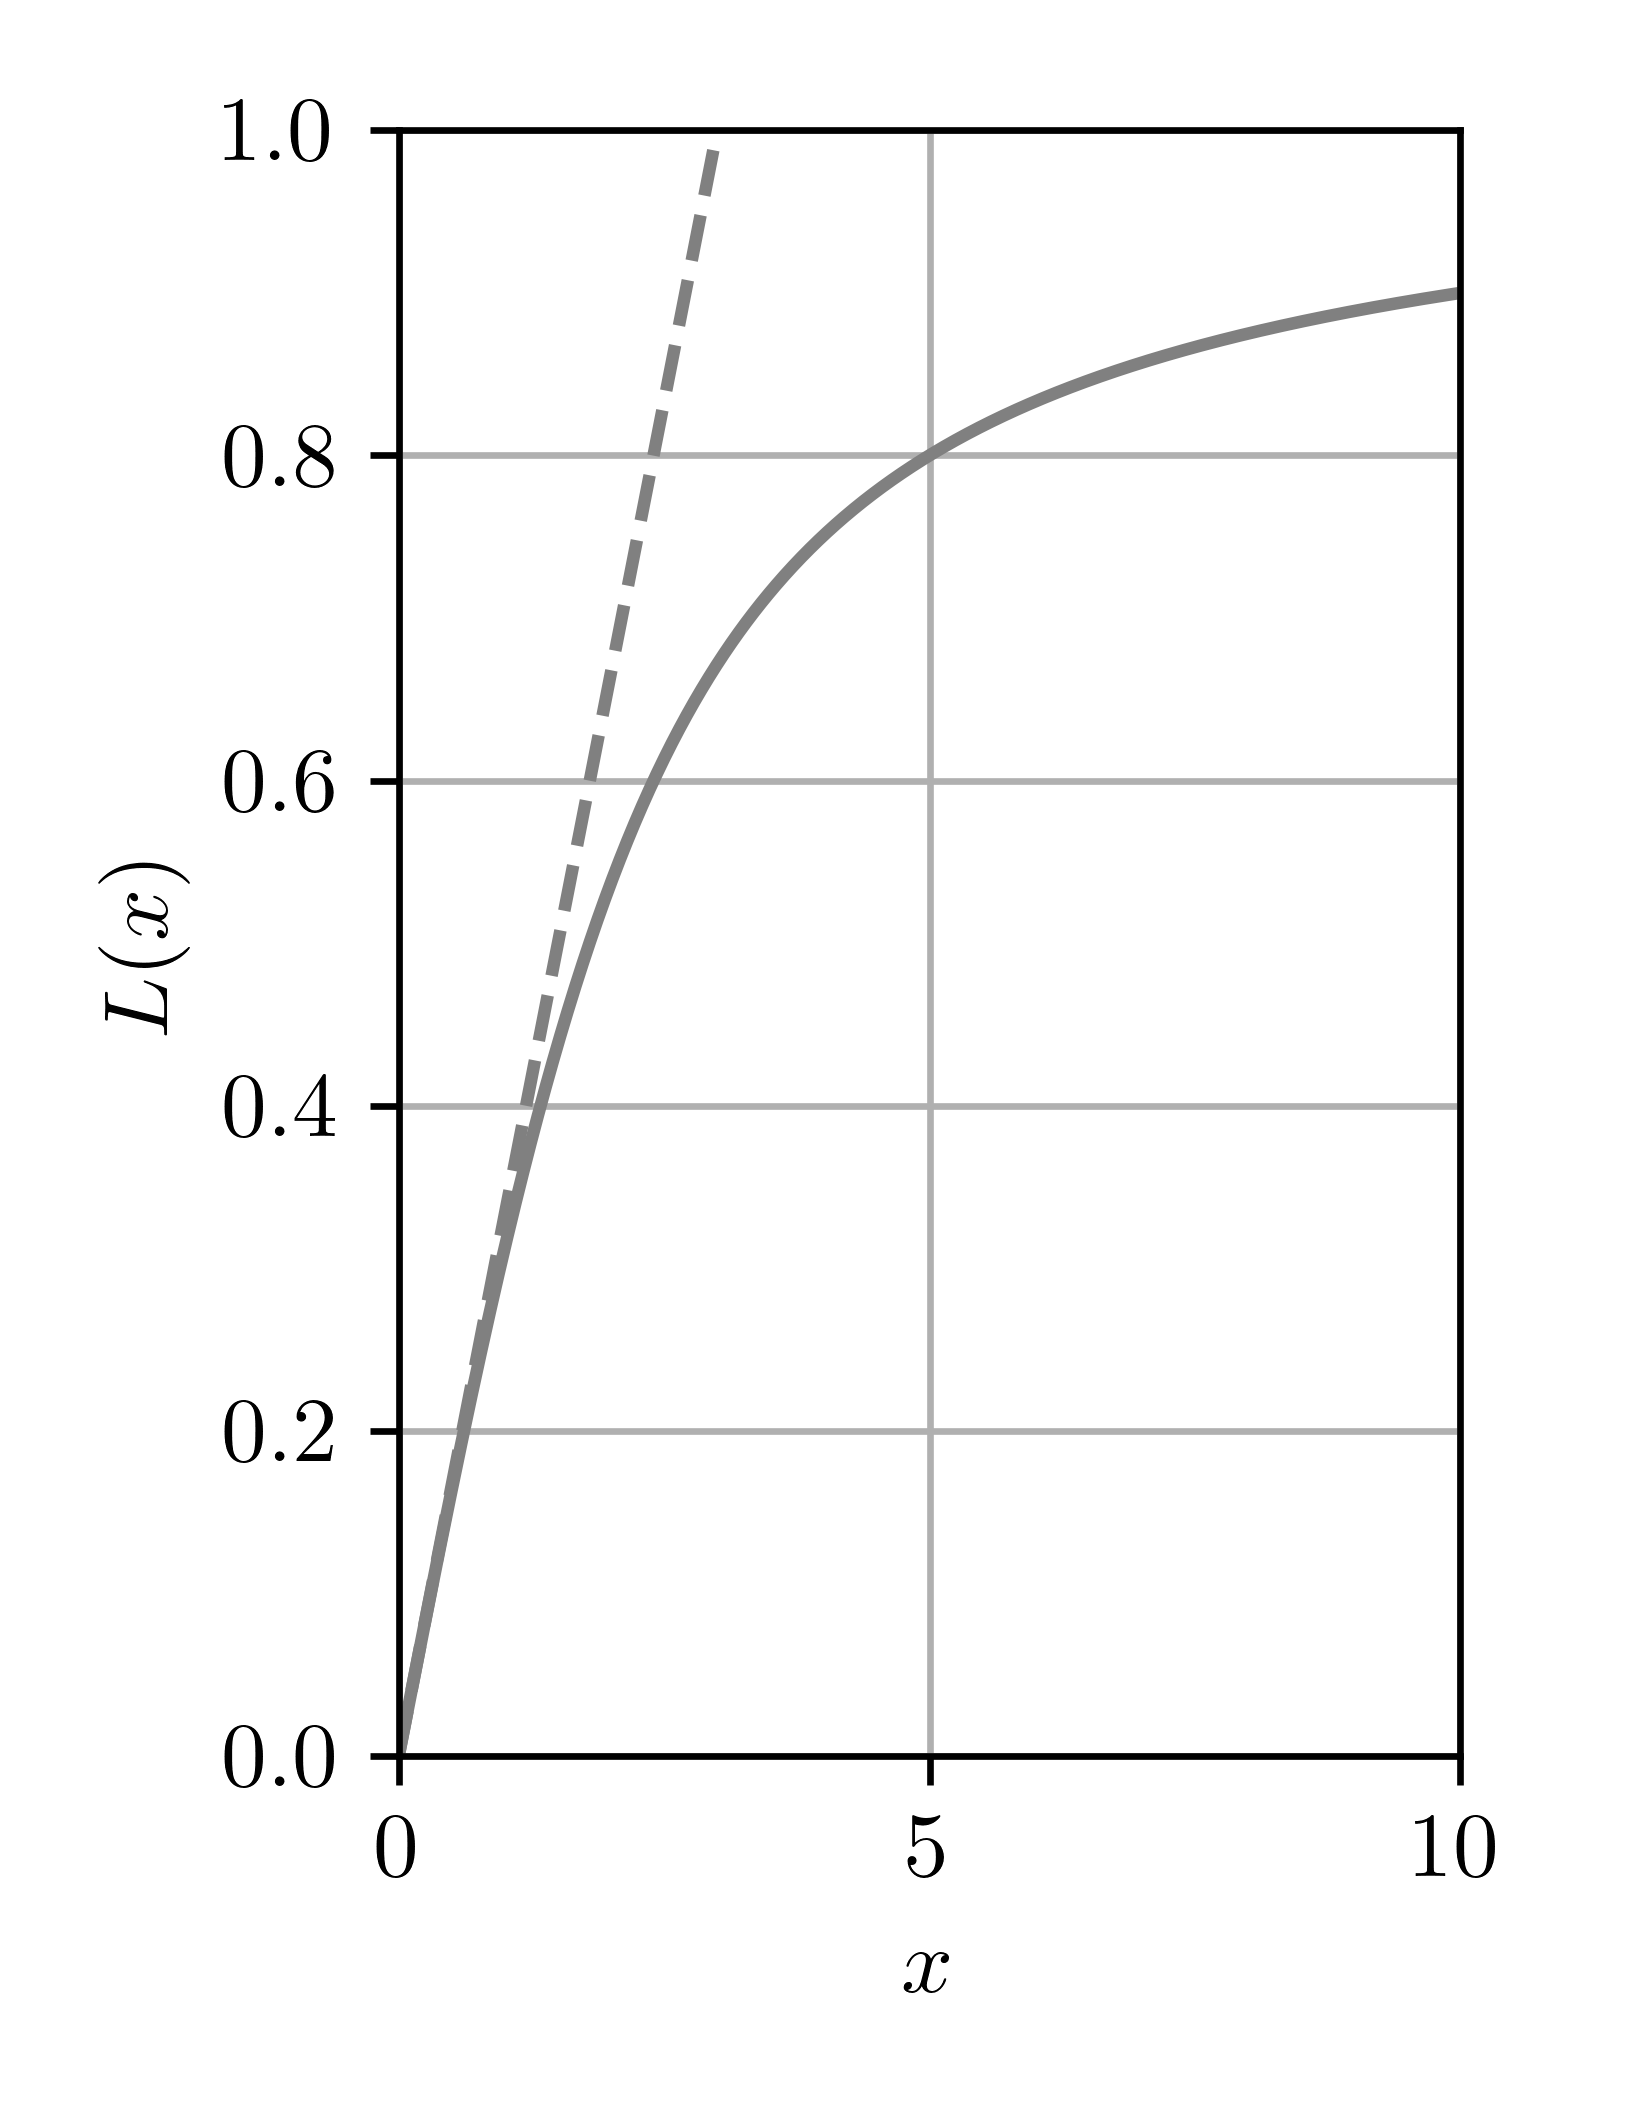
\includegraphics[width=\linewidth]{figures/vl2_langevin.jpg}
                \captionof{figure}{Langevin-Funktion $L(x)$ und gestrichelte lineare Approximation.}
                \label{fig:vl2_langevin}
            \end{verbal_sidebyside}
        
    	\item In verdünnten Gasen mit $ \varepsilon -1 \ll 1$ gilt mit \eqref{eq:2.3}, \eqref{eq:2.10} und \eqref{eq:2.16}
    		\begin{equation}
    			\label{2.17}
    			\varepsilon = 1 + N\Big( \underbrace{ \frac{\alpha}{ \varepsilon_0}}_{\text{induziert}} + \underbrace{ \frac{P_{p}^2}{3 \varepsilon_0 \mathrm{k}_{\mathrm{B}} T}}_{ \text{permanent}} \Big) = 1 + \chi 
    		\end{equation}
            
    \item Im Festkörper $\left( E _{\text{lok}} = E \right) $ gilt die 
        \begin{important}
            \textbf{Debye-Beziehung}\\
            \begin{equation}
    			\label{2.18}
    			\bm{\frac{ \varepsilon -1}{ \varepsilon +2} \frac{M}{ \rho} = \frac{1}{3 \varepsilon_0} \mathrm{N}_{\mathrm{A}} \left( \alpha + \frac{P_{p}^2 }{3 \mathrm{k}_{\mathrm{B}}T} \right) = P_{M}}
    		\end{equation}
        \end{important}
        anstelle der Clausius Mossotti-Gleichung (Rechnung analog).
    \end{itemize}

    \begin{verbal_sidebyside}[0.5\linewidth]
        Mithilfe von Messwerten wie in \autoref{fig:vl2_molpolarisierung} kann aus $\epsilon(T)$ die mikroskopischen Größen Polarisierbarkeit $\alpha$ und permanentes Dipolmoment $P_\text p$ mit der Debye-Beziehung \eqref{2.18} gefittet werden.\\

        Insbesondere fällt auf, dass unpolare Moleküle keine Steigung im Plot haben, da $P_\text P=0$ und somit der temperaturabhängige Teil der Debye-Beziehung \eqref{2.18} verschwindet.
        
        \tcblower
        \centering
        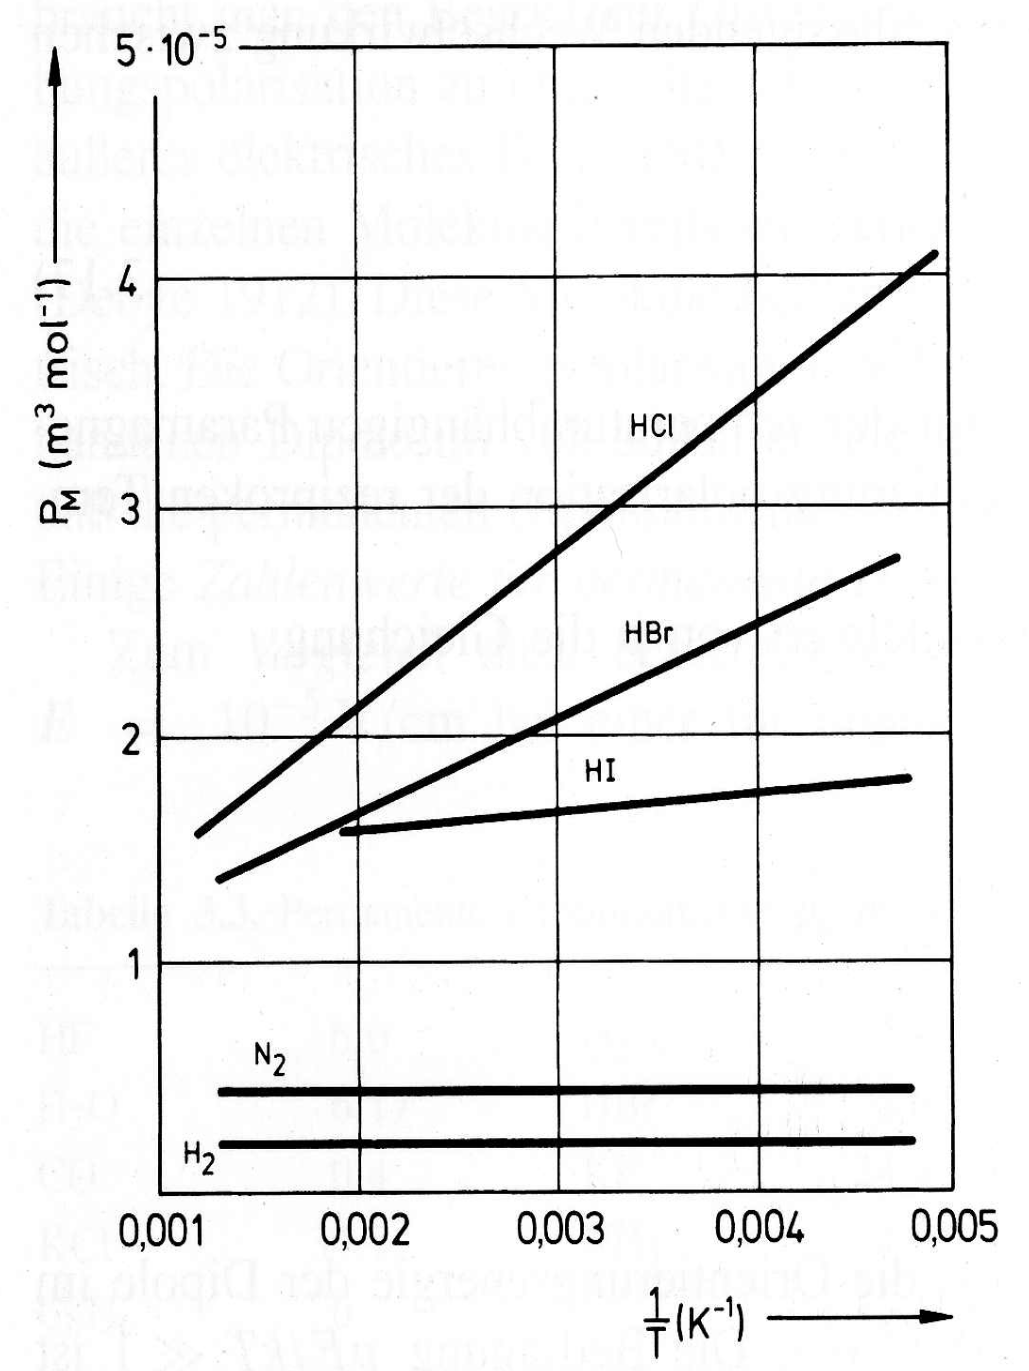
\includegraphics[width=\linewidth]{figures/vl2_molpolarisierung.png}
        \captionof{figure}{Molpolarisierung $P_\text M$ gegen die Temperaturinverse $\frac 1T$ für verschiedene Stoffe \cite{Haken_Wolf_2006}.}
        \label{fig:vl2_molpolarisierung}
    \end{verbal_sidebyside}

\paragraph{Bemerkung 2}
    Die charakteristische Zeit für die Umorientierung eines Moleküls entspricht der Zeit zur Rotation eines Moleküls $\left( \sim \SI{e-12}{s} \right)$. Also können Moleküle mit Frequenzen $\ge \SI{100}{\giga \hertz}$, wie dem Wechselfeld von Strahlung, aufgrund ihrer Trägheit nicht mehr mithalten.
